You are playing a tactical game and facing a brutal combat. 
Your rival's commander uses a circular formation to protect their headquarter, 
and you have to disrupt their defense to win the battle.
The enemy's circular formation consists of $n$ soldiers numbered from $1$ to $n$. 
In the beginning, soldier $i$ and soldier $j$ are 
adjacent if $|i-j|\in\{1,n-1\}$.
\begin{figure}[h]
\center
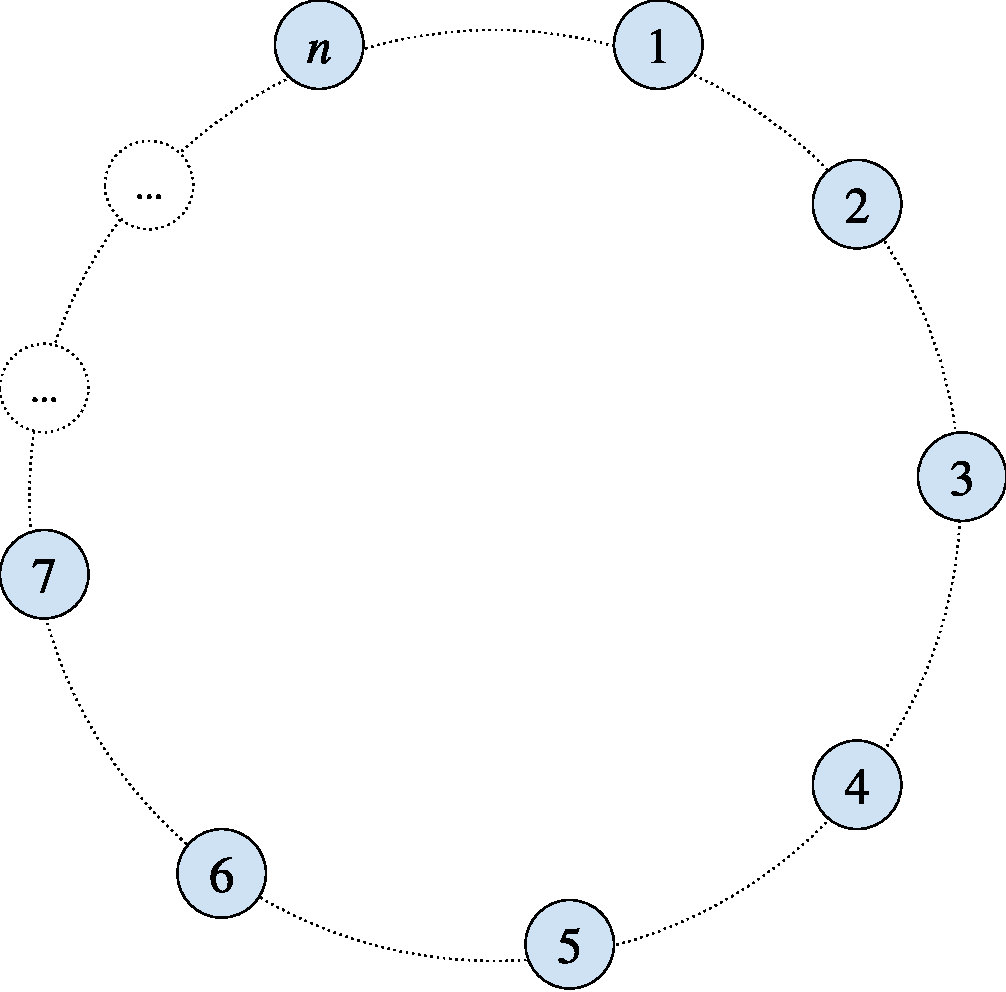
\includegraphics[width=5cm]{image/d-circle.pdf}
\end{figure}

You only have a small crew of warriors. 
Your force is too weak to fight more than two soldiers or any two soldiers
who are not adjacent. 
Moreover, if you try to attack a single soldier, both of their adjacent
soldiers will come to the rescue.
In such situation, it is equivalent to fighting three soldiers.
Thus, you may only launch attacks to aim at the gap between 
two adjacent soldiers.
By doing so, you have a chance to take down these two soldiers.
Your enemy will fill the gap after your attack. 
For example, soldiers $3$ and $n$ will become adjacent
if you take down soldiers $1$ and $2$.
You can repeatedly take down the soldiers until no one can defend 
their headquarter.

Unfortunately, you are still unable to defeat them in some situations.
Each of the soldiers has their own value, 
and there are at most $k$ different kinds of values in total.
You should have heard ``United we stand, divided we fall'' before. 
The soldiers with the same value can unite, 
and the soldiers with different values cannot.
When you attack two soldiers with different values, you always take them down.
But when you attack two soldiers with the same value, they will not fall.

Please write a program to find out an attacking strategy to win the battle
by disrupting the enemy's defense. That is, take down all $n$ soldiers
of the circular formation.
